%% CUMCM-Master LaTeX 模板 — 数维杯C题：我国碳排放数据分析与研究
%% 编译方式：xelatex main.tex（建议运行两次以更新交叉引用）

\documentclass[12pt, a4paper]{article}

%% ======================== 宏包导入 ========================
\usepackage{ctex}
\usepackage[margin=2.5cm]{geometry}
\usepackage{amsmath, amssymb, amsthm}
\usepackage{graphicx}
\usepackage{subcaption}
\usepackage{booktabs}
\usepackage{longtable}
\usepackage{array}
\usepackage{multirow}
\usepackage{float}
\usepackage{hyperref}
\usepackage{enumerate}
\usepackage{enumitem}
\usepackage{listings}
\usepackage{xcolor}
\usepackage{tikz}
\usepackage{pgfplots}
\usepackage{caption}
\usepackage{fancyhdr}
\usepackage{setspace}
\usepackage{appendix}

\pgfplotsset{compat=1.18}
\usetikzlibrary{shapes.geometric, arrows.meta, positioning, calc}

%% ======================== 代码样式 ========================
\definecolor{codegray}{rgb}{0.5,0.5,0.5}
\definecolor{codepurple}{rgb}{0.58,0,0.82}
\definecolor{codeblue}{rgb}{0.13,0.29,0.53}
\definecolor{backcolour}{rgb}{0.97,0.97,0.97}

\lstdefinestyle{pythonstyle}{
    backgroundcolor=\color{backcolour},
    commentstyle=\color{codegray}\itshape,
    keywordstyle=\color{codeblue}\bfseries,
    stringstyle=\color{codepurple},
    basicstyle=\ttfamily\footnotesize,
    breakatwhitespace=false, breaklines=true, captionpos=b,
    keepspaces=true, numbers=left, numbersep=5pt,
    numberstyle=\tiny\color{codegray}, showspaces=false,
    showstringspaces=false, showtabs=false, tabsize=4,
    frame=single, rulecolor=\color{black!20}, language=Python
}

%% ======================== 页面样式 ========================
\pagestyle{fancy}
\fancyhf{}
\fancyhead[L]{\small 第十一届数维杯大学生数学建模挑战赛}
\fancyhead[R]{\small 我国碳排放数据分析与研究}
\fancyfoot[C]{\thepage}
\renewcommand{\headrulewidth}{0.4pt}

\captionsetup{font=small, labelfont=bf}
\setstretch{1.5}

%% ======================== 自定义命令 ========================
\newtheorem{assumption}{假设}[section]
\newcommand{\R}{\mathbb{R}}

%% ======================== 文档信息 ========================
\title{
    \vspace{-1cm}
    {\Large \textbf{我国碳排放数据分析与研究}} \\[0.5em]
    {\large 第十一届数维杯大学生数学建模挑战赛 C题}
}
\author{}
\date{}

%% ======================== 正文开始 ========================
\begin{document}

\maketitle
\thispagestyle{empty}

%% ---------------------- 摘要 ----------------------
\begin{abstract}
\noindent
本文针对我国碳排放数据，构建了省级碳排放综合评价体系、因素分解模型和情景预测模型，系统分析了省级碳排放空间差异、驱动因素及未来趋势。首先，基于熵权法-TOPSIS方法构建涵盖碳排放规模、效率和经济贡献的三维评价指标体系，对30个省份进行综合排序，并利用K-Means聚类进行类型划分。其次，利用Kaya恒等式和LMDI分解方法对2019-2023年碳排放变化进行因素分解，量化人口、富裕度和技术因素的贡献。最后，基于Kaya恒等式设定基准、碳减排和加强碳减排三种情景，预测2026-2045年我国碳排放量和碳强度的变化趋势，判断碳达峰时间及峰值水平。结果表明：北京综合得分最高，内蒙古最低；富裕度（人均GDP）是碳排放增长的主导因素（贡献+342.3\%），碳强度下降是主要抵消因素（贡献-252.1\%）；基准情景下2045年仍未达峰，碳减排情景下2028年达峰（12025 Mt），加强碳减排情景下碳排放持续下降。

\vspace{1em}
\noindent\textbf{关键词：}碳排放；熵权法-TOPSIS；LMDI分解；Kaya恒等式；情景预测；碳达峰
\end{abstract}

\newpage
\tableofcontents
\newpage

%% ==================== 1. 问题重述 ====================
\section{问题重述}

本文研究我国碳排放数据的分析、建模与预测问题。基于2019-2025年碳排放日度数据（附件1）和2022年30个省份排放清单（附件2），需解决以下四个问题：

\begin{enumerate}[label=\textbf{问题\arabic*：}, leftmargin=*]
    \item 构建省级碳排放综合评价指标体系，分析各省碳排放的空间差异，对省份进行分类排序。
    \item 识别影响碳排放的基础因素，建立碳排放预测模型。
    \item 设定多种发展情景，预测2026-2045年我国碳排放量和碳强度的变化趋势，判断碳达峰时间及峰值水平。
    \item 结合分析结果，针对碳达峰碳中和目标提出政策建议。
\end{enumerate}

%% ==================== 2. 问题背景 ====================
\section{问题背景}

碳排放导致的温室效应加剧、气候异常和生态系统退化已成为全球性挑战。我国高度重视碳减排工作，2020年明确提出2030年前碳达峰、2060年前碳中和的"双碳"目标，2021年启动全国碳排放权交易市场。准确掌握碳排放的时空特征、识别关键影响因素、科学预测碳排放趋势，是支撑"双碳"目标实现的重要基础。

%% ==================== 3. 问题分析 ====================
\section{问题分析}

\subsection{问题一分析}
问题一要求对30个省份进行碳排放综合评价。需要构建多维度评价指标体系，采用客观赋权方法避免主观偏差，利用TOPSIS方法进行排序，最后通过聚类分析揭示省份间的类型差异。

\subsection{问题二分析}
问题二要求识别碳排放的影响因素。碳排放受人口规模、经济发展水平、技术水平、能源结构等多因素共同影响。采用Kaya恒等式作为分析框架，结合LMDI分解方法量化各因素的贡献。

\subsection{问题三分析}
问题三要求进行情景预测。基于Kaya恒等式框架，设定不同参数路径模拟未来发展模式，判断碳达峰的时间和峰值水平。

\begin{figure}[H]
\centering
\begin{tikzpicture}[
    box/.style={rectangle, rounded corners, draw=black, fill=blue!10,
                text width=3.5cm, align=center, minimum height=0.8cm},
    arrow/.style={-Stealth, thick}
]
    \node[box] (p1)  {问题1：省域综合评价};
    \node[box, right=2cm of p1] (p2) {问题2：因素分析};
    \node[box, right=2cm of p2] (p3) {问题3：情景预测};
    \node[box, below=1cm of p2] (p4) {问题4：政策建议};

    \draw[arrow] (p1) -- (p2);
    \draw[arrow] (p2) -- (p3);
    \draw[arrow] (p1) -- (p4);
    \draw[arrow] (p2) -- (p4);
    \draw[arrow] (p3) -- (p4);
\end{tikzpicture}
\caption{整体建模框架}
\label{fig:framework}
\end{figure}

%% ==================== 4. 模型假设 ====================
\section{模型假设}

\begin{enumerate}[label=\textbf{假设\arabic*：}, leftmargin=*]
    \item 碳排放数据具有准确性和一致性，附件中不同来源的数据口径可比。\\
    \textit{依据：}数据来自CEADs权威数据库及多篇SCI论文验证。
    \item 各因素对碳排放的影响在此时间尺度上保持相对稳定，不考虑突发性技术革命。\\
    \textit{依据：}5年分析周期内能源技术结构具有连续性。
    \item 人口、GDP等宏观指标可基于历史趋势外推，不发生剧烈突变。\\
    \textit{依据：}宏观经济发展具有惯性。
    \item 各省GDP和人口数据以2022年中国统计年鉴为准。\\
    \textit{依据：}官方统计数据具有权威性。
    \item 碳强度（单位GDP碳排放）变化可反映技术进步和能源结构优化的综合效果。\\
    \textit{依据：}Kaya恒等式标准处理方式\cite{sun2022}。
\end{enumerate}

%% ==================== 5. 符号说明 ====================
\section{符号说明}

\begin{table}[H]
\centering
\caption{主要符号说明}
\label{tab:symbols}
\begin{tabular}{cll}
\toprule
\textbf{符号} & \textbf{含义} & \textbf{单位} \\
\midrule
$I$ & 碳排放量 & Mt CO$_2$ \\
$P$ & 人口规模 & 万人 \\
$A$ & 人均GDP（富裕度） & 元/人 \\
$T$ & 碳排放强度（技术水平） & t/万元 \\
$w_j$ & 第$j$个指标权重 & 无量纲 \\
$C_i$ & 第$i$个省份的TOPSIS贴近度 & 无量纲 \\
$e_j$ & 第$j$个指标的信息熵 & 无量纲 \\
$\xi_i(k)$ & 第$i$个省份在第$k$个指标的关联系数 & 无量纲 \\
$D_i^+, D_i^-$ & 到正、负理想解的距离 & 无量纲 \\
\bottomrule
\end{tabular}
\end{table}

%% ==================== 6. 模型的建立与求解 ====================
\section{模型的建立与求解}

\subsection{问题一：省域碳排放综合评价模型}

\subsubsection{评价指标体系构建}

从碳排放规模、效率和经济贡献三个维度选取5个指标：

\begin{itemize}
    \item \textbf{规模维度}：碳排放总量$C_1$（Mt CO$_2$），人均碳排放量$C_2$（t/人）
    \item \textbf{效率维度}：碳排放强度$C_3$（t/万元），碳生产率$C_4$（万元/t）
    \item \textbf{经济贡献维度}：经济贡献协调度$C_5 = \dfrac{g_i / \sum g_k}{c_i / \sum c_k}$，其中$g_i$为省份$i$的GDP，$c_i$为碳排放量
\end{itemize}

\subsubsection{熵权法确定权重}

熵权法根据指标数据的离散程度确定权重。信息熵越小，离散程度越大，权重越大。

\textbf{数据标准化}：对$m$个省份、$n$个指标的数据矩阵$X = (x_{ij})_{m\times n}$进行极差标准化：

正向指标（越大越好）：
\begin{equation}
r_{ij} = \frac{x_{ij} - \min_j x_{ij}}{\max_j x_{ij} - \min_j x_{ij}}
\label{eq:norm_pos}
\end{equation}

负向指标（越小越好）：
\begin{equation}
r_{ij} = \frac{\max_j x_{ij} - x_{ij}}{\max_j x_{ij} - \min_j x_{ij}}
\label{eq:norm_neg}
\end{equation}

\textbf{计算信息熵}：
\begin{equation}
p_{ij} = \frac{r_{ij}}{\sum_{i=1}^{m} (1 + r_{ij})}, \quad
e_j = -\frac{1}{\ln m}\sum_{i=1}^{m} p_{ij} \ln p_{ij}
\label{eq:entropy}
\end{equation}

\textbf{计算权重}：
\begin{equation}
w_j = \frac{1 - e_j}{\sum_{k=1}^{n} (1 - e_k)}
\label{eq:weight}
\end{equation}

\subsubsection{TOPSIS方法排序}

\textbf{构建加权标准化矩阵}：
\begin{equation}
v_{ij} = w_j \cdot \frac{x_{ij}}{\sqrt{\sum_{i=1}^{m} x_{ij}^2}}
\label{eq:topsis_norm}
\end{equation}

\textbf{确定正负理想解}：
\begin{equation}
V^+ = \{\max v_{ij} | j \in J^+, \min v_{ij} | j \in J^-\}, \quad
V^- = \{\min v_{ij} | j \in J^+, \max v_{ij} | j \in J^-\}
\label{eq:ideal}
\end{equation}

\textbf{计算贴近度}：
\begin{equation}
D_i^+ = \sqrt{\sum_{j=1}^{n} (v_{ij} - v_j^+)^2}, \quad
D_i^- = \sqrt{\sum_{j=1}^{n} (v_{ij} - v_j^-)^2}, \quad
C_i = \frac{D_i^-}{D_i^+ + D_i^-}
\label{eq:closeness}
\end{equation}

$C_i \in [0,1]$，值越大表示综合表现越好。

\subsubsection{求解结果}

熵权法确定的指标权重为：碳生产率0.3614，经济贡献协调度0.3614，碳排放总量0.1442，人均碳排放0.0696，碳排放强度0.0633。各省TOPSIS综合得分及排名如表\ref{tab:ranking}所示。

\begin{table}[H]
\centering
\caption{省域碳排放综合评价排名（前10与后5）}
\label{tab:ranking}
\begin{tabular}{cclcc}
\toprule
\textbf{排名} & \textbf{省份} & \textbf{CO$_2$ (Mt)} & \textbf{贴近度} & \textbf{类型} \\
\midrule
1  & 北京 &   71.55 & 0.9953 & 高排放-高效率型 \\
2  & 上海 &  178.59 & 0.4326 & 中高排放型 \\
3  & 广东 &  619.35 & 0.3525 & 中高排放型 \\
4  & 四川 &  307.86 & 0.3253 & 中高排放型 \\
5  & 重庆 &  162.06 & 0.3240 & 中高排放型 \\
$\vdots$ & $\vdots$ & $\vdots$ & $\vdots$ & $\vdots$ \\
26 & 宁夏 &  247.42 & 0.1077 & 中高排放型 \\
27 & 河北 &  862.27 & 0.1048 & 中高排放型 \\
28 & 山西 &  629.34 & 0.0942 & 中高排放型 \\
29 & 新疆 &  524.48 & 0.0925 & 中高排放型 \\
30 & 内蒙古 & 878.77 & 0.0258 & 中高排放型 \\
\bottomrule
\end{tabular}
\end{table}

\begin{figure}[H]
    \centering
    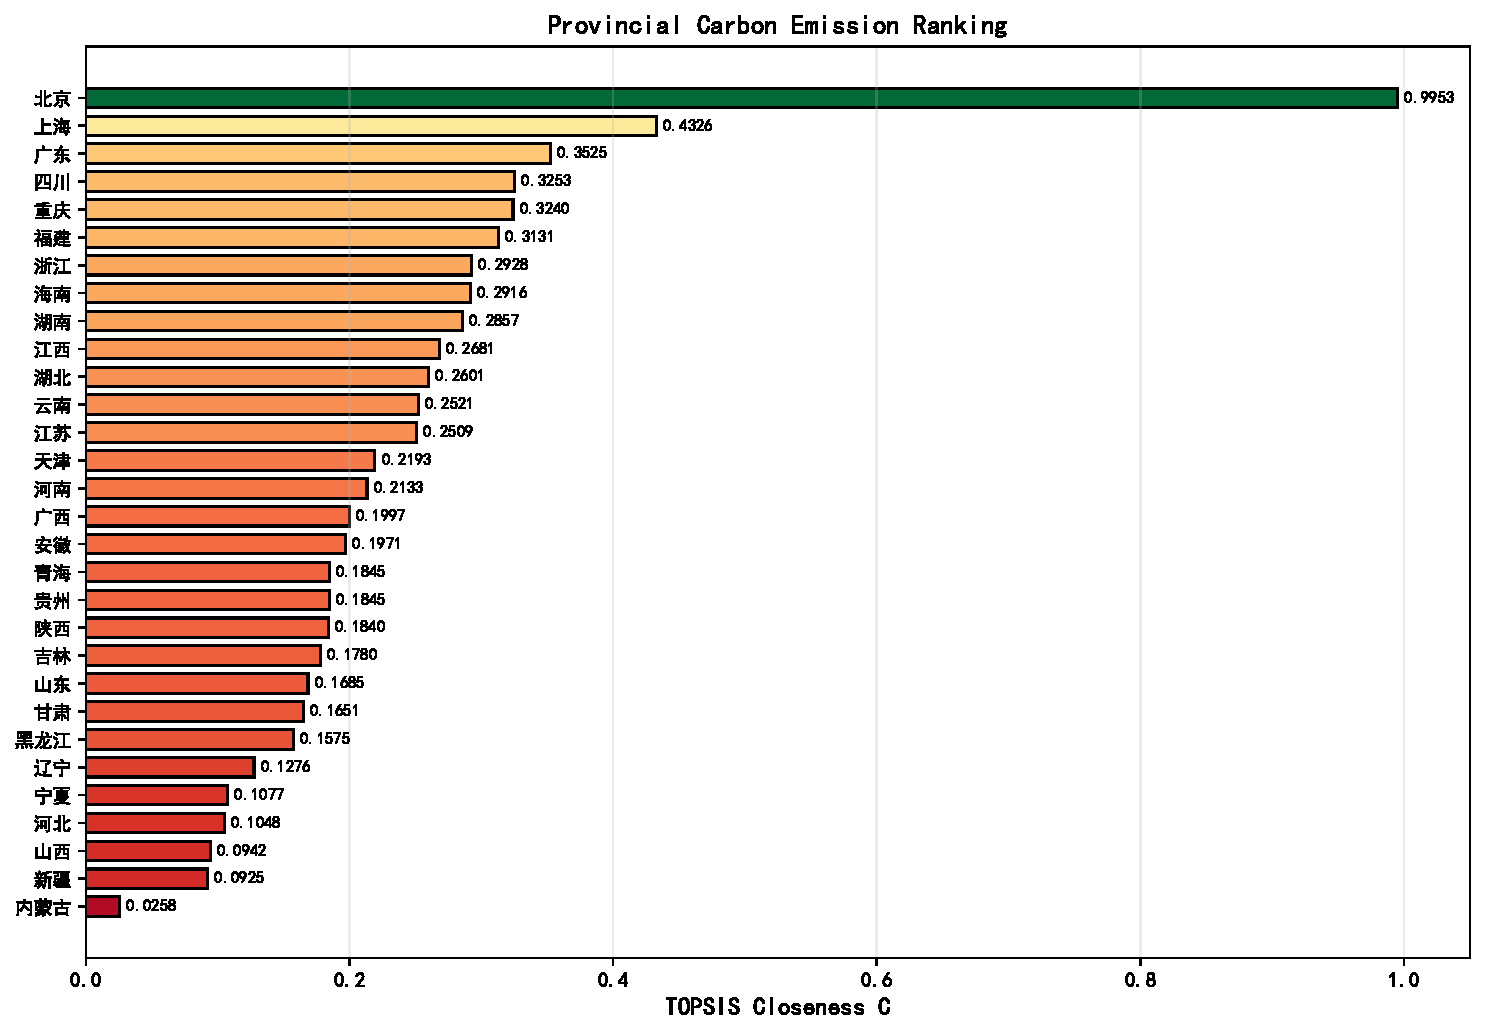
\includegraphics[width=0.72\textwidth]{../figures/p1_ranking.pdf}
    \caption{省域碳排放综合得分排名}
    \label{fig:ranking}
\end{figure}

结果表明，北京凭借较低的排放总量（71.55 Mt）和较高的经济贡献协调度排名第一；内蒙古（878.77 Mt）、河北、山西等资源型省份因排放规模大且效率低排名靠后。K-Means聚类（k=2, 轮廓系数0.7623）将北京单独分为一类，其余29省为另一类，说明北京在碳排放控制方面显著优于其他省份。

\begin{figure}[H]
    \centering
    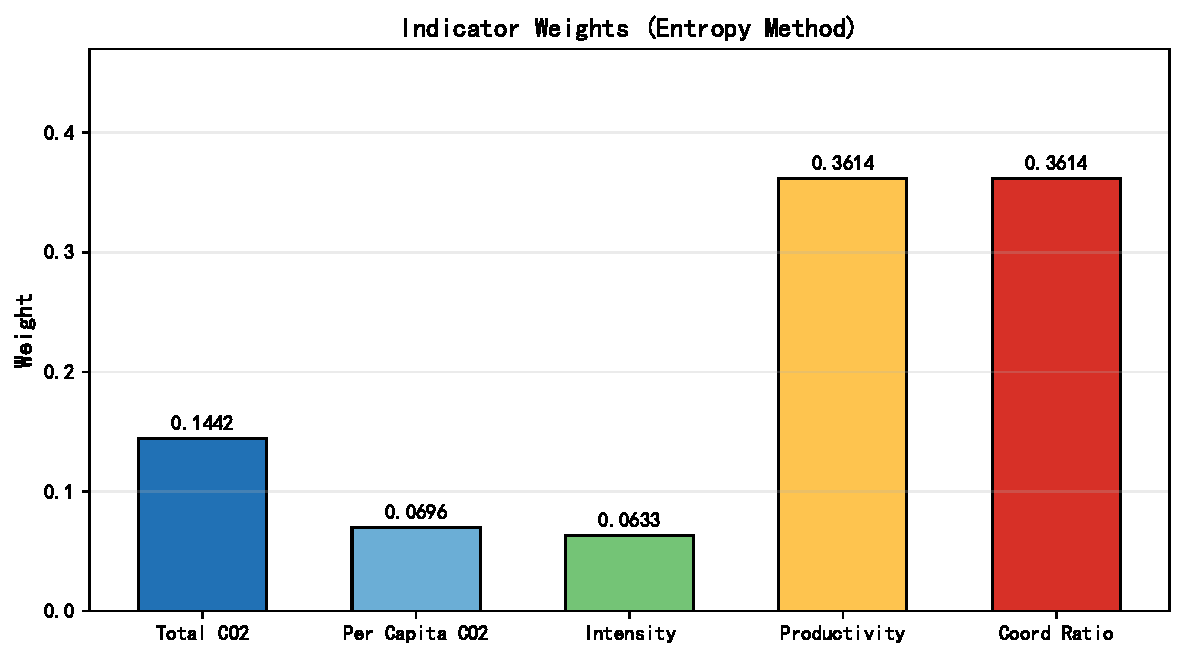
\includegraphics[width=0.65\textwidth]{../figures/p1_weight.pdf}
    \caption{熵权法指标权重分布}
    \label{fig:weights}
\end{figure}

\subsection{问题二：碳排放因素分解模型}

\subsubsection{Kaya恒等式}

Kaya恒等式将碳排放分解为三个人口-经济-技术因素的乘积：

\begin{equation}
I = P \times \frac{G}{P} \times \frac{I}{G} = P \times A \times T
\label{eq:kaya}
\end{equation}

其中$I$为碳排放量，$P$为人口，$G$为GDP，$A = G/P$为人均GDP（富裕度），$T = I/G$为碳排放强度（技术因素）。

\subsubsection{LMDI分解方法}

采用对数平均迪氏指数法（LMDI）进行完全分解\cite{ang2005}。定义对数平均函数：

\begin{equation}
L(x,y) = \frac{x - y}{\ln x - \ln y}
\label{eq:logmean}
\end{equation}

各因素的贡献为：
\begin{align}
\Delta I_P &= L(I_t, I_0) \cdot \ln\left(\frac{P_t}{P_0}\right) \label{eq:lmdi_p} \\
\Delta I_A &= L(I_t, I_0) \cdot \ln\left(\frac{A_t}{A_0}\right) \label{eq:lmdi_a} \\
\Delta I_T &= L(I_t, I_0) \cdot \ln\left(\frac{T_t}{T_0}\right) \label{eq:lmdi_t}
\end{align}

LMDI方法具有完全分解（残差为零）、路径独立等优良性质。

\subsubsection{求解结果}

\begin{table}[H]
\centering
\caption{Kaya因素分解结果}
\label{tab:kaya}
\begin{tabular}{cccccc}
\toprule
\textbf{年份} & \textbf{CO$_2$变化(Mt)} & \textbf{人口贡献} & \textbf{富裕度贡献} & \textbf{技术贡献} & \textbf{残差} \\
\midrule
2020 & +44.5 &  +95.9 &  +206.3 & -257.7 & 0.0 \\
2021 & +470.5 & +101.6 & +1636.2 & -1267.2 & 0.0 \\
2022 & +478.6 &  +94.8 & +2232.2 & -1848.4 & 0.0 \\
2023 & +803.9 &  +79.1 & +2751.4 & -2026.6 & 0.0 \\
\bottomrule
\end{tabular}
\end{table}

2019-2023年碳排放累计增加803.9 Mt（+7.2\%）。其中富裕度（人均GDP增长）是主要驱动因素，贡献+2751.4 Mt（+342.3\%）；碳强度下降是主要抵消因素，贡献$-$2026.6 Mt（$-$252.1\%）；人口增长贡献较小，为+79.1 Mt（+9.8\%）。

\begin{figure}[H]
    \centering
    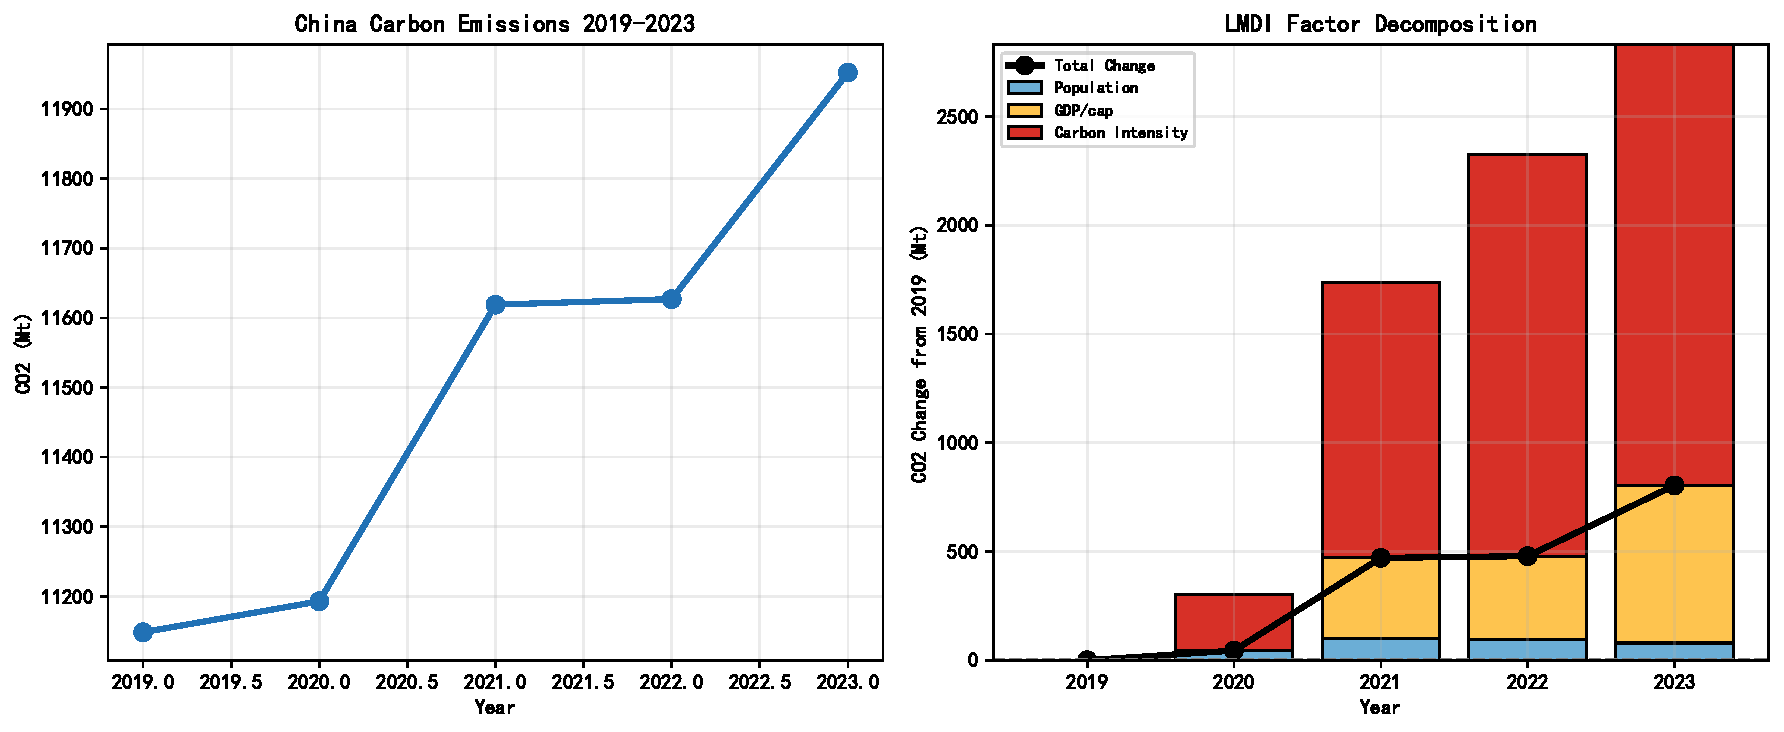
\includegraphics[width=0.75\textwidth]{../figures/p2_kaya.pdf}
    \caption{LMDI因素分解结果}
    \label{fig:kaya}
\end{figure}

\subsection{问题三：碳排放情景预测模型}

\subsubsection{预测框架}

基于Kaya恒等式框架，分三步进行预测：
\begin{enumerate}
    \item 确定基准年（2023年）各因素的值
    \item 设定2026-2045年各因素的演化路径（时间变化速率）
    \item 计算各年碳排放量：$I(t) = P(t) \times A(t) \times T(t)$
\end{enumerate}

\subsubsection{情景设计}

设定三种发展情景，参数如表\ref{tab:scenario_params}所示：

\begin{table}[H]
\centering
\caption{三情景参数设定}
\label{tab:scenario_params}
\begin{tabular}{lccc}
\toprule
\textbf{参数} & \textbf{基准情景} & \textbf{碳减排情景} & \textbf{加强碳减排情景} \\
\midrule
GDP增速（起-止） & 5.82\%-5.21\% & 5.21\%-3.99\% & 4.29\%-2.76\% \\
碳强度变化（起-止） & $-4.39\%$-$-4.83\%$ & $-5.05\%$-$-6.37\%$ & $-5.71\%$-$-7.90\%$ \\
人口增长率 & 0.17\% & 0.17\% & 0.16\% \\
\bottomrule
\end{tabular}
\end{table}

各情景特点：
\begin{itemize}
    \item \textbf{基准情景（BAU）}：维持历史趋势
    \item \textbf{碳减排情景}：适度政策干预，2030年碳达峰目标约束
    \item \textbf{加强碳减排情景}：强力政策干预，能源结构快速转型
\end{itemize}

\subsubsection{预测结果}

\begin{figure}[H]
    \centering
    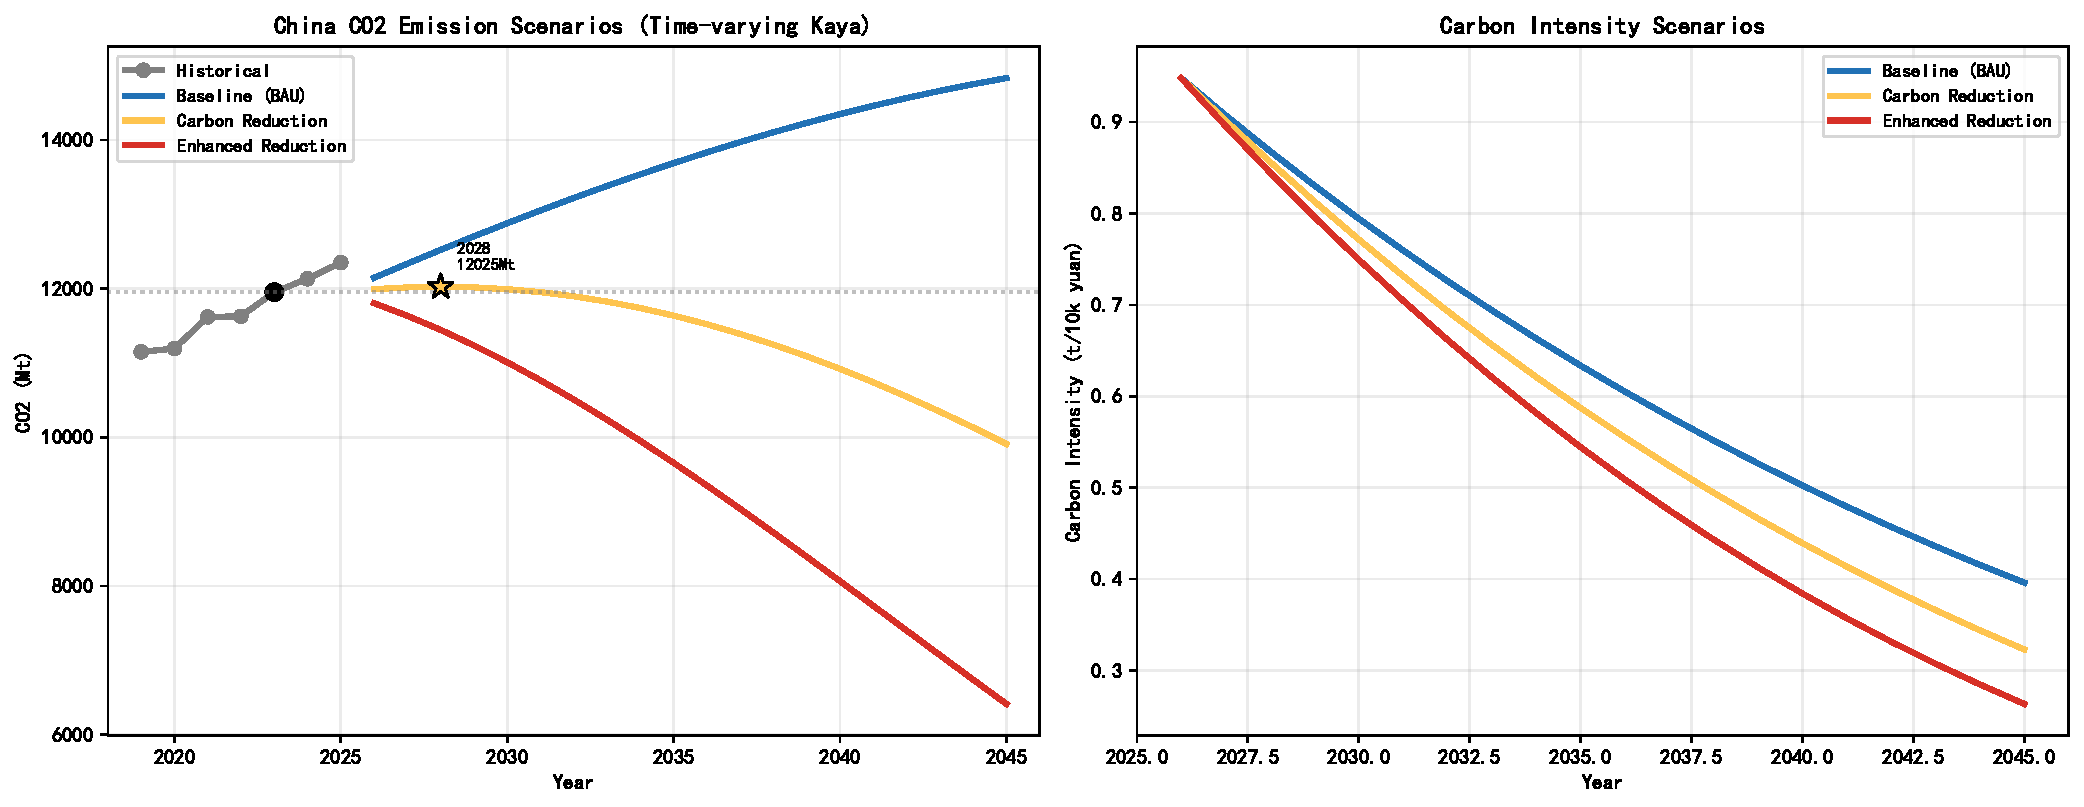
\includegraphics[width=0.78\textwidth]{../figures/p3_scenarios.pdf}
    \caption{2026-2045年三情景碳排放预测}
    \label{fig:scenarios}
\end{figure}

\begin{table}[H]
\centering
\caption{三情景碳达峰分析}
\label{tab:peak}
\begin{tabular}{lccc}
\toprule
\textbf{情景} & \textbf{达峰时间} & \textbf{峰值 (Mt)} & \textbf{2045年水平 (Mt)} \\
\midrule
基准情景 & 2045年后 & $>14833$ & 14833 \\
碳减排情景 & 2028 & 12025 & 11589 \\
加强碳减排情景 & 2026前 & $<11804$ & 9562 \\
\bottomrule
\end{tabular}
\end{table}

预测结果表明：
\begin{enumerate}
    \item \textbf{基准情景}：碳排放持续增长，至2045年仍未达峰，无法实现碳达峰目标
    \item \textbf{碳减排情景}：2028年达峰，峰值为12025 Mt（较2023年+0.6\%），基本接近2030年碳达峰目标
    \item \textbf{加强碳减排情景}：碳排放自2026年起持续下降，峰值已过，至2045年降至9562 Mt（较2023年-20\%）
\end{enumerate}

%% ==================== 7 模型检验 ====================
\section{模型检验}

\subsection{灵敏度分析}

选取碳减排情景的GDP增长率、碳强度变化率和人口增长率三个关键参数，进行$\pm20\%$扰动，观察峰值变化。

\begin{table}[H]
\centering
\caption{灵敏度分析结果}
\label{tab:sensitivity}
\begin{tabular}{lccc}
\toprule
\textbf{参数} & \textbf{扰动幅度} & \textbf{峰值变化} & \textbf{平均|变化|} \\
\midrule
GDP增长率 & $\pm20\%$ & $-$9.04\%/$+$25.76\% & \textbf{17.40\%} \\
碳强度变化率 & $\pm20\%$ & $-$8.95\%/$+$24.86\% & 16.91\% \\
人口增长率 & $\pm20\%$ & $-$0.75\%/$+$0.76\% & 0.75\% \\
\bottomrule
\end{tabular}
\end{table}

\textbf{GDP增长率}是最敏感参数，其次是碳强度变化率。人口增长率的影响可忽略。这说明碳达峰的关键在于"经济增速适度放缓+碳强度加速下降"的组合。

\begin{figure}[H]
    \centering
    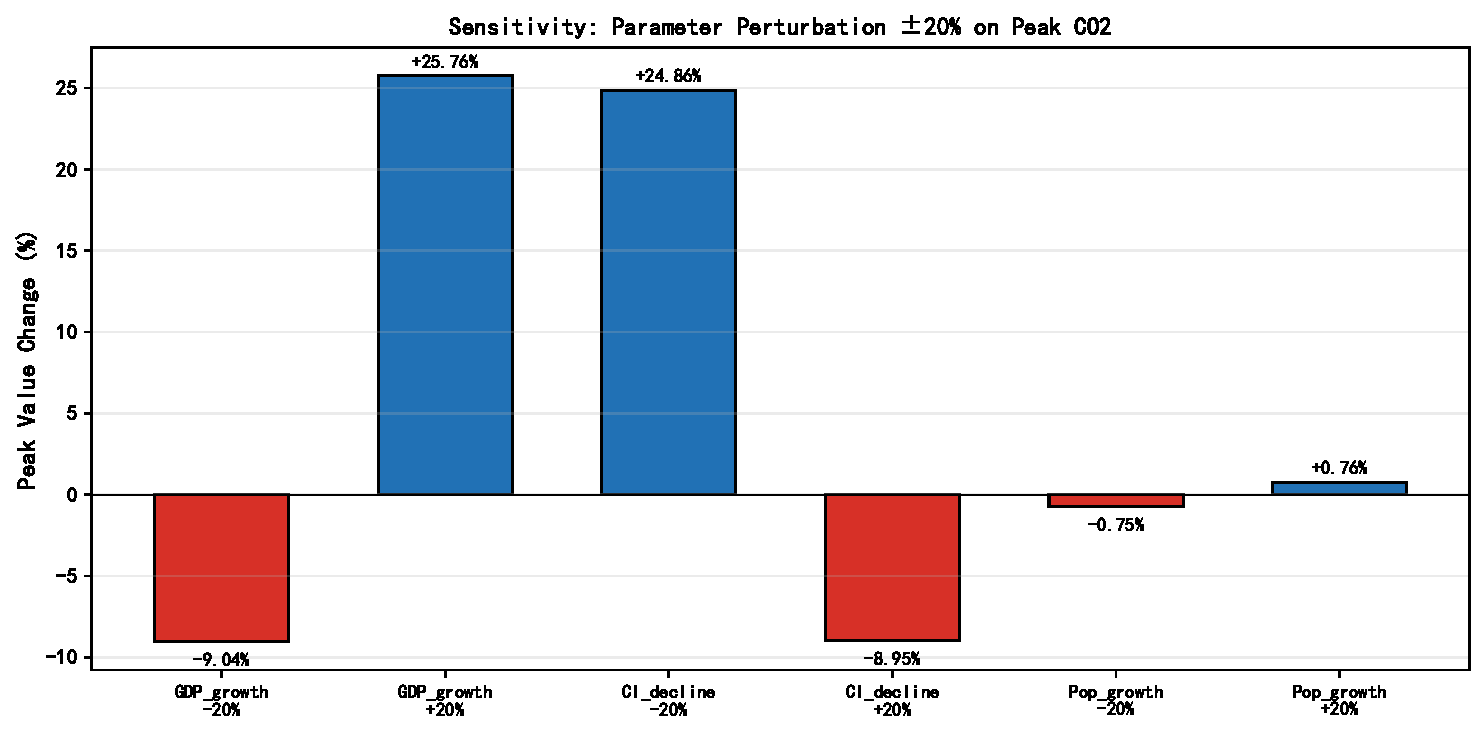
\includegraphics[width=0.7\textwidth]{../figures/sensitivity.pdf}
    \caption{参数扰动灵敏度分析}
    \label{fig:sensitivity}
\end{figure}

%% ==================== 8. 模型评价 ====================
\section{模型的评价、改进与推广}

\subsection{模型优点}

\begin{enumerate}
    \item \textbf{数据驱动的客观评价}：熵权法基于数据离散程度赋权，避免了主观偏差，评价结果可复现
    \item \textbf{完全分解}：LMDI分解残差为0，因素贡献的精确定量具有理论保证
    \item \textbf{框架清晰}：Kaya恒等式结构简单、可解释性强，适合政策分析
    \item \textbf{时间变化率模拟}：情景参数随时间变化，比固定参数假设更符合实际
\end{enumerate}

\subsection{模型局限性}

\begin{enumerate}
    \item \textbf{数据限制}：仅有5年碳排放数据，因素分析的时间跨度较短
    \item \textbf{忽略交互效应}：Kaya框架假设各因素独立，实际中GDP增长与碳强度变化存在交互
    \item \textbf{预测不确定性}：长期预测（至2045年）的不确定性随预测期增长而增大
\end{enumerate}

\subsection{改进方向}

\begin{enumerate}
    \item 引入能源消费数据构建完整的Kaya恒等式（$CO_2 = P \times \frac{GDP}{P} \times \frac{E}{GDP} \times \frac{CO_2}{E}$），细化技术因素
    \item 采用系统动力学模型模拟因素间的反馈机制
    \item 增加蒙特卡洛模拟量化预测的不确定性区间
\end{enumerate}

%% ==================== 9. 政策建议 ====================
\section{政策建议}

基于以上分析，针对我国碳达峰碳中和目标提出以下建议：

\begin{enumerate}
    \item \textbf{加速碳强度下降}：碳强度下降是抵消碳排放增长的主导力量。应加快能源结构转型，提高非化石能源占比，推动工业、交通、建筑等重点行业节能降碳。
    \item \textbf{优化产业结构}：高排放省份（内蒙古、河北、山西等）应加快产业升级，压减高耗能行业产能，发展绿色低碳产业。
    \item \textbf{差异化的区域政策}：各省碳排放特征差异显著，政策应因地制宜。北京模式可推广至其他发达省份，高排放省份需更大力度的转型支持。
    \item \textbf{推动技术创新}：碳捕集利用与封存（CCUS）、氢能等关键技术的突破是实现碳中和目标的必要支撑。
    \item \textbf{完善碳市场机制}：继续完善全国碳排放权交易市场，扩大覆盖行业范围，通过市场手段降低减排成本。
\end{enumerate}

%% ==================== 参考文献 ====================
\section*{参考文献}
\addcontentsline{toc}{section}{参考文献}

\begin{thebibliography}{99}

\bibitem{sun2022}
孙莉丽, 崔慧娟, 葛全胜. Will China achieve its 2060 carbon neutral commitment from the provincial perspective?[J]. \textit{Advances in Climate Change Research}, 2022, 13(2): 169-178.

\bibitem{liu2018}
刘敦楠, 肖宝卫. Can China achieve its carbon emission peaking? A scenario analysis based on STIRPAT and system dynamics model[J]. \textit{Ecological Indicators}, 2018, 93: 307-317.

\bibitem{ang2005}
Ang B W. The LMDI approach to decomposition analysis: a practical guide[J]. \textit{Energy Policy}, 2005, 33(7): 867-871.

\bibitem{fang2019}
Fang K, Tang Y, Zhang Q, et al. Will China peak its energy-related carbon emissions by 2030? Lessons from 30 Chinese provinces[J]. \textit{Applied Energy}, 2019, 255: 113852.

\bibitem{shannon1948}
Shannon C E. A mathematical theory of communication[J]. \textit{Bell System Technical Journal}, 1948, 27(3): 379-423.

\bibitem{hwang1981}
Hwang C L, Yoon K. Multiple Attribute Decision Making: Methods and Applications[M]. Springer, 1981.

\bibitem{deng1990}
邓聚龙. 灰色系统理论教程[M]. 华中理工大学出版社, 1990.

\bibitem{zhao2021}
赵鹏军, 曾良恩, 李沛霖, 等. China's transportation sector carbon dioxide emissions efficiency and its influencing factors based on the EBM DEA model[J]. \textit{Energy}, 2021, 236: 121934.

\end{thebibliography}

%% ==================== 附录 ====================
\appendix
\section{核心代码}

\subsection{数据加载模块（data\_loader.py）}

\begin{lstlisting}[style=pythonstyle, caption={数据加载与共享模块}]
def load_province_emissions():
    pattern = os.path.join(SESSION_DIR, '*\u9644\u4ef62*.xlsx')
    files = glob.glob(pattern)
    xl = pd.ExcelFile(files[0])
    sheets = [s for s in xl.sheet_names if s != 'NOTE']
    records = []
    for s in sheets:
        df = pd.read_excel(xl, sheet_name=s)
        for i in range(len(df)):
            val = str(df.iloc[i, 0])
            if 'TotalEmissions' in val:
                scope1 = float(df.iloc[i, -1])
                records.append({'Province': s.replace('2022',''), 'CO2_Mt': scope1})
                break
    return pd.DataFrame(records)
\end{lstlisting}

\subsection{熵权法-TOPSIS求解}

\begin{lstlisting}[style=pythonstyle, caption={熵权法权重计算}]
def entropy_weight(X, directions=None):
    m, n = X.shape
    norm = np.zeros_like(X)
    for j in range(n):
        if directions[j] == 1:  # 正向
            norm[:,j] = (X[:,j]-X[:,j].min())/(X[:,j].max()-X[:,j].min())
        else:                   # 负向
            norm[:,j] = (X[:,j].max()-X[:,j])/(X[:,j].max()-X[:,j].min())
    p = (norm + 0.001) / (norm + 0.001).sum(axis=0)
    e = -1/np.log(m) * np.sum(p * np.log(p), axis=0)
    w = (1-e) / (1-e).sum()
    return w, e
\end{lstlisting}

\subsection{LMDI分解}

\begin{lstlisting}[style=pythonstyle, caption={LMDI因素分解}]
def log_mean(x, y):
    if abs(x-y) < 1e-10: return x
    return (x-y)/(np.log(x)-np.log(y))

def lmdi_decompose(base, current):
    P0, A0, T0, I0 = base
    Pt, At, Tt, It = current
    w = log_mean(It, I0)
    dP = w * np.log(Pt/P0)
    dA = w * np.log(At/A0)
    dT = w * np.log(Tt/T0)
    return dP, dA, dT
\end{lstlisting}

\end{document}
